\scanpage{74}
\[\unsure{S_i}\mathcal T_{0,I}\qquad \mathcal T_{0,I}\qquad i_0\ \uline{I}\qquad i'_1\ne i'_0\]
\[i_0\deleted{\unsure{i}}\in I\setminus\{i_1\}
= i_0\amalg\unsure{(I\setminus\{i_0,i_1\})}\]
\[\deleted{\unsure{\pi^2}}\]
\diagram{\begin{tikzcd}[ampersand replacement=\&]\mathcal T_{0,I}\arrow[d,"\unsure{\pi_1}"]\\\mathcal T_{0,I\setminus\{i_1\}}\end{tikzcd}}
\figure{\begin{tikzpicture}\draw (0,0)--(.7,1.6);\end{tikzpicture}}
\diagram{\begin{tikzcd}[ampersand replacement=\&]M_{0,K}\arrow[d]\\M_{0,I}\end{tikzcd}}
\[\unsure{\mathcal T}\qquad \times\quad 1\ 2\ 3\ 4\qquad 5\]
\[H\qquad \unsure{\mathcal O(}\qquad
\mathcal O(4)^{\unsure{\otimes}}\,\deleted{\uline{\unsure{degrés}}}\simeq\mathcal O(-2)\simeq\Omega^1\]
\[\prod_{i\in I}\deleted{\unsure{\mathcal O}}L_i\]
\[H^1(\widetilde G_5,M^!_{0,5};G_m).\qquad
M_{0,I}\hookrightarrow\prod_{i\in\deleted{K}}\uline{\Sigma_{J(i)}}\qquad I\setminus\{i\}\]
\[H^1(M_{0,5};G_m)\simeq 0\]
\[H^0(M^!_{0,5},G_m)\qquad \uline{M_{0,5}}\]
\unsure{à coups d'éclatements}

\[H^2(\mathcal T^+_{0,5},\mathbb Z)=\qquad :\ \text{\unsure{partir de}}\quad\mathbb P_1\times\mathbb P_1\]
\[\unsure{H^1(M^!_{0,5}}\]
\figure{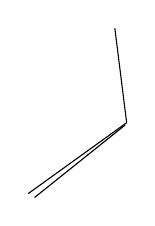
\begin{tikzpicture}\draw (1.1,2.1)--(1.25,.9)--(0,0);\draw (1.23,.87)--(.08,-.05);\end{tikzpicture}}
\diagram{\begin{tikzcd}[ampersand replacement=\&]M^!_{0,5}\arrow[d]\&\unsure{-}\&U_{0,3}\times U_{0,3}\arrow[d]\\M^!_{0,4}\simeq U_{0,3}\&\&U_{0,3}\end{tikzcd}}
\[H^0(U_{0,3},G_m)\qquad\unsure{21}\qquad\unsure{\ne}\]
\figure{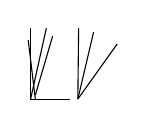
\begin{tikzpicture}\draw (0,.9)--(0,0)--(.5,0);\draw (0,0)--(.2,.9);\draw (.06,0)--(-.03,.75);\draw (.06,.05)--(.28,.8);\draw (.6,0)--(.61,.9);\draw (.6,0)--(.8,.85);\draw (.6,0)--(1.1,.7);\end{tikzpicture}}
\diagram{\begin{tikzcd}[ampersand replacement=\&, column sep=small]0\arrow[r]\&G_m\arrow[r]\&H^0(M^{\unsure{\partial}}_{0,\deleted{K}},G_m)\arrow[r]\&(\mathbb Z^{P_3(K)})'\arrow[r,dash]\&0\end{tikzcd}}
\diagram{\begin{tikzcd}[ampersand replacement=\&, column sep=small]
0\arrow[r,dash]\&\underbrace{H^1(\widetilde G_K,G_m)}_{\unsure{\pm1}}\arrow[r]\&\underbrace{H^1(\widetilde G_K,H^0(M_{0,K},G_m))}_{\unsure{H^1(M_{0,n},\widetilde G_n;G_m)}}\arrow[r]\&H^1(\widetilde G_{\unsure{5}},(\mathbb Z^{P_3(K)})')\arrow[d]\\\&\&\&H^2(\widetilde G_n,\unsure{G_m})
\end{tikzcd}}
\mspage{73}
